\documentclass[1p]{elsarticle_modified}
%\bibliographystyle{elsarticle-num}

%\usepackage[colorlinks]{hyperref}
%\usepackage{abbrmath_seonhwa} %\Abb, \Ascr, \Acal ,\Abf, \Afrak
\usepackage{amsfonts}
\usepackage{amssymb}
\usepackage{amsmath}
\usepackage{amsthm}
\usepackage{scalefnt}
\usepackage{amsbsy}
\usepackage{kotex}
\usepackage{caption}
\usepackage{subfig}
\usepackage{color}
\usepackage{graphicx}
\usepackage{xcolor} %% white, black, red, green, blue, cyan, magenta, yellow
\usepackage{float}
\usepackage{setspace}
\usepackage{hyperref}

\usepackage{tikz}
\usetikzlibrary{arrows}

\usepackage{multirow}
\usepackage{array} % fixed length table
\usepackage{hhline}

%%%%%%%%%%%%%%%%%%%%%
\makeatletter
\renewcommand*\env@matrix[1][\arraystretch]{%
	\edef\arraystretch{#1}%
	\hskip -\arraycolsep
	\let\@ifnextchar\new@ifnextchar
	\array{*\c@MaxMatrixCols c}}
\makeatother %https://tex.stackexchange.com/questions/14071/how-can-i-increase-the-line-spacing-in-a-matrix
%%%%%%%%%%%%%%%

\usepackage[normalem]{ulem}

\newcommand{\msout}[1]{\ifmmode\text{\sout{\ensuremath{#1}}}\else\sout{#1}\fi}
%SOURCE: \msout is \stkout macro in https://tex.stackexchange.com/questions/20609/strikeout-in-math-mode

\newcommand{\cancel}[1]{
	\ifmmode
	{\color{red}\msout{#1}}
	\else
	{\color{red}\sout{#1}}
	\fi
}

\newcommand{\add}[1]{
	{\color{blue}\uwave{#1}}
}

\newcommand{\replace}[2]{
	\ifmmode
	{\color{red}\msout{#1}}{\color{blue}\uwave{#2}}
	\else
	{\color{red}\sout{#1}}{\color{blue}\uwave{#2}}
	\fi
}

\newcommand{\Sol}{\mathcal{S}} %segment
\newcommand{\D}{D} %diagram
\newcommand{\A}{\mathcal{A}} %arc


%%%%%%%%%%%%%%%%%%%%%%%%%%%%%5 test

\def\sl{\operatorname{\textup{SL}}(2,\Cbb)}
\def\psl{\operatorname{\textup{PSL}}(2,\Cbb)}
\def\quan{\mkern 1mu \triangleright \mkern 1mu}

\theoremstyle{definition}
\newtheorem{thm}{Theorem}[section]
\newtheorem{prop}[thm]{Proposition}
\newtheorem{lem}[thm]{Lemma}
\newtheorem{ques}[thm]{Question}
\newtheorem{cor}[thm]{Corollary}
\newtheorem{defn}[thm]{Definition}
\newtheorem{exam}[thm]{Example}
\newtheorem{rmk}[thm]{Remark}
\newtheorem{alg}[thm]{Algorithm}

\newcommand{\I}{\sqrt{-1}}
\begin{document}

%\begin{frontmatter}
%
%\title{Boundary parabolic representations of knots up to 8 crossings}
%
%%% Group authors per affiliation:
%\author{Yunhi Cho} 
%\address{Department of Mathematics, University of Seoul, Seoul, Korea}
%\ead{yhcho@uos.ac.kr}
%
%
%\author{Seonhwa Kim} %\fnref{s_kim}}
%\address{Center for Geometry and Physics, Institute for Basic Science, Pohang, 37673, Korea}
%\ead{ryeona17@ibs.re.kr}
%
%\author{Hyuk Kim}
%\address{Department of Mathematical Sciences, Seoul National University, Seoul 08826, Korea}
%\ead{hyukkim@snu.ac.kr}
%
%\author{Seokbeom Yoon}
%\address{Department of Mathematical Sciences, Seoul National University, Seoul, 08826,  Korea}
%\ead{sbyoon15@snu.ac.kr}
%
%\begin{abstract}
%We find all boundary parabolic representation of knots up to 8 crossings.
%
%\end{abstract}
%\begin{keyword}
%    \MSC[2010] 57M25 
%\end{keyword}
%
%\end{frontmatter}

%\linenumbers
%\tableofcontents
%
\newcommand\colored[1]{\textcolor{white}{\rule[-0.35ex]{0.8em}{1.4ex}}\kern-0.8em\color{red} #1}%
%\newcommand\colored[1]{\textcolor{white}{ #1}\kern-2.17ex	\textcolor{white}{ #1}\kern-1.81ex	\textcolor{white}{ #1}\kern-2.15ex\color{red}#1	}

{\Large $\underline{12n_{0372}~(K12n_{0372})}$}

\setlength{\tabcolsep}{10pt}
\renewcommand{\arraystretch}{1.6}
\vspace{1cm}\begin{tabular}{m{100pt}>{\centering\arraybackslash}m{274pt}}
\multirow{5}{120pt}{
	\centering
	\includegraphics[width=112pt]{../../../GIT/diagram.site/Diagrams/png/2461_12n_0372.png}\\
\ \ \ A knot diagram\footnotemark}&
\allowdisplaybreaks
\textbf{Linearized knot diagam} \\
\cline{2-2}
 &
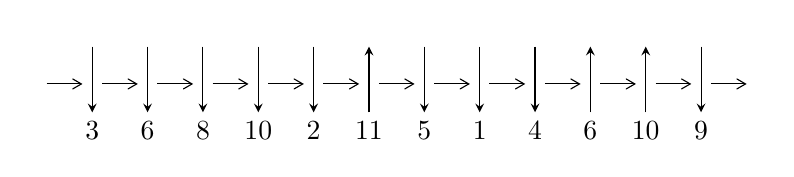
\begin{tikzpicture}[x=20pt, y=17pt]
	% nodes
	\node (C0) at (0, 0) {};
	\node (C1) at (1, 0) {};
	\node (C1U) at (1, +1) {};
	\node (C1D) at (1, -1) {3};

	\node (C2) at (2, 0) {};
	\node (C2U) at (2, +1) {};
	\node (C2D) at (2, -1) {6};

	\node (C3) at (3, 0) {};
	\node (C3U) at (3, +1) {};
	\node (C3D) at (3, -1) {8};

	\node (C4) at (4, 0) {};
	\node (C4U) at (4, +1) {};
	\node (C4D) at (4, -1) {10};

	\node (C5) at (5, 0) {};
	\node (C5U) at (5, +1) {};
	\node (C5D) at (5, -1) {2};

	\node (C6) at (6, 0) {};
	\node (C6U) at (6, +1) {};
	\node (C6D) at (6, -1) {11};

	\node (C7) at (7, 0) {};
	\node (C7U) at (7, +1) {};
	\node (C7D) at (7, -1) {5};

	\node (C8) at (8, 0) {};
	\node (C8U) at (8, +1) {};
	\node (C8D) at (8, -1) {1};

	\node (C9) at (9, 0) {};
	\node (C9U) at (9, +1) {};
	\node (C9D) at (9, -1) {4};

	\node (C10) at (10, 0) {};
	\node (C10U) at (10, +1) {};
	\node (C10D) at (10, -1) {6};

	\node (C11) at (11, 0) {};
	\node (C11U) at (11, +1) {};
	\node (C11D) at (11, -1) {10};

	\node (C12) at (12, 0) {};
	\node (C12U) at (12, +1) {};
	\node (C12D) at (12, -1) {9};
	\node (C13) at (13, 0) {};

	% arrows
	\draw[->,>={angle 60}]
	(C0) edge (C1) (C1) edge (C2) (C2) edge (C3) (C3) edge (C4) (C4) edge (C5) (C5) edge (C6) (C6) edge (C7) (C7) edge (C8) (C8) edge (C9) (C9) edge (C10) (C10) edge (C11) (C11) edge (C12) (C12) edge (C13) ;	\draw[->,>=stealth]
	(C1U) edge (C1D) (C2U) edge (C2D) (C3U) edge (C3D) (C4U) edge (C4D) (C5U) edge (C5D) (C6D) edge (C6U) (C7U) edge (C7D) (C8U) edge (C8D) (C9U) edge (C9D) (C10D) edge (C10U) (C11D) edge (C11U) (C12U) edge (C12D) ;
	\end{tikzpicture} \\
\hhline{~~} \\& 
\textbf{Solving Sequence} \\ \cline{2-2} 
 &
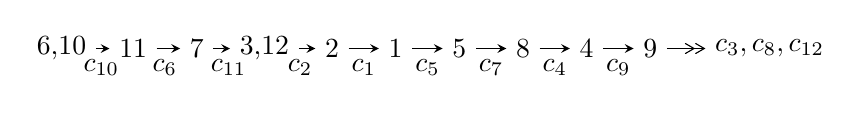
\begin{tikzpicture}[x=23pt, y=7pt]
	% node
	\node (A0) at (-1/8, 0) {6,10};
	\node (A1) at (1, 0) {11};
	\node (A2) at (2, 0) {7};
	\node (A3) at (49/16, 0) {3,12};
	\node (A4) at (33/8, 0) {2};
	\node (A5) at (41/8, 0) {1};
	\node (A6) at (49/8, 0) {5};
	\node (A7) at (57/8, 0) {8};
	\node (A8) at (65/8, 0) {4};
	\node (A9) at (73/8, 0) {9};
	\node (C1) at (1/2, -1) {$c_{10}$};
	\node (C2) at (3/2, -1) {$c_{6}$};
	\node (C3) at (5/2, -1) {$c_{11}$};
	\node (C4) at (29/8, -1) {$c_{2}$};
	\node (C5) at (37/8, -1) {$c_{1}$};
	\node (C6) at (45/8, -1) {$c_{5}$};
	\node (C7) at (53/8, -1) {$c_{7}$};
	\node (C8) at (61/8, -1) {$c_{4}$};
	\node (C9) at (69/8, -1) {$c_{9}$};
	\node (A10) at (11, 0) {$c_{3},c_{8},c_{12}$};

	% edge
	\draw[->,>=stealth]	
	(A0) edge (A1) (A1) edge (A2) (A2) edge (A3) (A3) edge (A4) (A4) edge (A5) (A5) edge (A6) (A6) edge (A7) (A7) edge (A8) (A8) edge (A9) ;
	\draw[->>,>={angle 60}]	
	(A9) edge (A10);
\end{tikzpicture} \\ 

\end{tabular} \\

\footnotetext{
The image of knot diagram is generated by the software ``\textbf{Draw programme}" developed by Andrew Bartholomew(\url{http://www.layer8.co.uk/maths/draw/index.htm\#Running-draw}), where we modified some parts for our purpose(\url{https://github.com/CATsTAILs/LinksPainter}).
}\phantom \\ \newline 
\centering \textbf{Ideals for irreducible components\footnotemark of $X_{\text{par}}$} 
 
\begin{align*}
I^u_{1}&=\langle 
1.42529\times10^{92} u^{36}+8.72680\times10^{91} u^{35}+\cdots+1.49513\times10^{93} b+2.35282\times10^{95},\\
\phantom{I^u_{1}}&\phantom{= \langle  }-3.02051\times10^{94} u^{36}-1.75541\times10^{94} u^{35}+\cdots+6.54608\times10^{94} a-5.25852\times10^{97},\\
\phantom{I^u_{1}}&\phantom{= \langle  }u^{37}-30 u^{35}+\cdots+4671 u-1007\rangle \\
I^u_{2}&=\langle 
7 u^{14}-13 u^{13}+\cdots+b+17,\;-13 u^{15}+34 u^{14}+\cdots+a+20,\;u^{16}-3 u^{15}+\cdots-4 u+1\rangle \\
\\
\end{align*}
\raggedright * 2 irreducible components of $\dim_{\mathbb{C}}=0$, with total 53 representations.\\
\footnotetext{All coefficients of polynomials are rational numbers. But the coefficients are sometimes approximated in decimal forms when there is not enough margin.}
\newpage
\renewcommand{\arraystretch}{1}
\centering \section*{I. $I^u_{1}= \langle 1.43\times10^{92} u^{36}+8.73\times10^{91} u^{35}+\cdots+1.50\times10^{93} b+2.35\times10^{95},\;-3.02\times10^{94} u^{36}-1.76\times10^{94} u^{35}+\cdots+6.55\times10^{94} a-5.26\times10^{97},\;u^{37}-30 u^{35}+\cdots+4671 u-1007 \rangle$}
\flushleft \textbf{(i) Arc colorings}\\
\begin{tabular}{m{7pt} m{180pt} m{7pt} m{180pt} }
\flushright $a_{6}=$&$\begin{pmatrix}0\\u\end{pmatrix}$ \\
\flushright $a_{10}=$&$\begin{pmatrix}1\\0\end{pmatrix}$ \\
\flushright $a_{11}=$&$\begin{pmatrix}1\\- u^2\end{pmatrix}$ \\
\flushright $a_{7}=$&$\begin{pmatrix}u\\- u^3+u\end{pmatrix}$ \\
\flushright $a_{3}=$&$\begin{pmatrix}0.461422 u^{36}+0.268162 u^{35}+\cdots-2340.32 u+803.308\\-0.0953284 u^{36}-0.0583680 u^{35}+\cdots+476.203 u-157.365\end{pmatrix}$ \\
\flushright $a_{12}=$&$\begin{pmatrix}- u^2+1\\- u^2\end{pmatrix}$ \\
\flushright $a_{2}=$&$\begin{pmatrix}0.461422 u^{36}+0.268162 u^{35}+\cdots-2340.32 u+803.308\\-0.250593 u^{36}-0.148286 u^{35}+\cdots+1264.14 u-427.405\end{pmatrix}$ \\
\flushright $a_{1}=$&$\begin{pmatrix}0.0803873 u^{36}+0.0415081 u^{35}+\cdots-433.347 u+161.373\\-0.176241 u^{36}-0.103850 u^{35}+\cdots+897.957 u-302.093\end{pmatrix}$ \\
\flushright $a_{5}=$&$\begin{pmatrix}-0.0247048 u^{36}-0.00822526 u^{35}+\cdots+139.528 u-59.8522\\0.304235 u^{36}+0.170592 u^{35}+\cdots-1563.50 u+546.853\end{pmatrix}$ \\
\flushright $a_{8}=$&$\begin{pmatrix}0.326831 u^{36}+0.178171 u^{35}+\cdots-1699.82 u+603.957\\-0.293525 u^{36}-0.170056 u^{35}+\cdots+1484.90 u-508.106\end{pmatrix}$ \\
\flushright $a_{4}=$&$\begin{pmatrix}0.279530 u^{36}+0.162367 u^{35}+\cdots-1423.97 u+487.001\\0.304235 u^{36}+0.170592 u^{35}+\cdots-1563.50 u+546.853\end{pmatrix}$ \\
\flushright $a_{9}=$&$\begin{pmatrix}-0.325873 u^{36}-0.178662 u^{35}+\cdots+1668.53 u-591.318\\0.169109 u^{36}+0.102532 u^{35}+\cdots-850.133 u+281.907\end{pmatrix}$\\&\end{tabular}
\flushleft \textbf{(ii) Obstruction class $= -1$}\\~\\
\flushleft \textbf{(iii) Cusp Shapes $= 1.65322 u^{36}+0.965871 u^{35}+\cdots-8351.56 u+2824.79$}\\~\\
\newpage\renewcommand{\arraystretch}{1}
\flushleft \textbf{(iv) u-Polynomials at the component}\newline \\
\begin{tabular}{m{50pt}|m{274pt}}
Crossings & \hspace{64pt}u-Polynomials at each crossing \\
\hline $$\begin{aligned}c_{1}\end{aligned}$$&$\begin{aligned}
&u^{37}+7 u^{36}+\cdots+33 u+1
\end{aligned}$\\
\hline $$\begin{aligned}c_{2},c_{5}\end{aligned}$$&$\begin{aligned}
&u^{37}+u^{36}+\cdots-5 u+1
\end{aligned}$\\
\hline $$\begin{aligned}c_{3}\end{aligned}$$&$\begin{aligned}
&u^{37}+u^{36}+\cdots-23 u-5
\end{aligned}$\\
\hline $$\begin{aligned}c_{4},c_{9}\end{aligned}$$&$\begin{aligned}
&u^{37}+3 u^{35}+\cdots-294 u-229
\end{aligned}$\\
\hline $$\begin{aligned}c_{6},c_{10}\end{aligned}$$&$\begin{aligned}
&u^{37}-30 u^{35}+\cdots+4671 u+1007
\end{aligned}$\\
\hline $$\begin{aligned}c_{7}\end{aligned}$$&$\begin{aligned}
&u^{37}-7 u^{36}+\cdots-207584 u-176401
\end{aligned}$\\
\hline $$\begin{aligned}c_{8},c_{12}\end{aligned}$$&$\begin{aligned}
&u^{37}-6 u^{36}+\cdots+3 u+1
\end{aligned}$\\
\hline $$\begin{aligned}c_{11}\end{aligned}$$&$\begin{aligned}
&u^{37}-60 u^{36}+\cdots+36901087 u-1014049
\end{aligned}$\\
\hline
\end{tabular}\\~\\
\newpage\renewcommand{\arraystretch}{1}
\flushleft \textbf{(v) Riley Polynomials at the component}\newline \\
\begin{tabular}{m{50pt}|m{274pt}}
Crossings & \hspace{64pt}Riley Polynomials at each crossing \\
\hline $$\begin{aligned}c_{1}\end{aligned}$$&$\begin{aligned}
&y^{37}+53 y^{36}+\cdots+369 y-1
\end{aligned}$\\
\hline $$\begin{aligned}c_{2},c_{5}\end{aligned}$$&$\begin{aligned}
&y^{37}-7 y^{36}+\cdots+33 y-1
\end{aligned}$\\
\hline $$\begin{aligned}c_{3}\end{aligned}$$&$\begin{aligned}
&y^{37}+3 y^{36}+\cdots-131 y-25
\end{aligned}$\\
\hline $$\begin{aligned}c_{4},c_{9}\end{aligned}$$&$\begin{aligned}
&y^{37}+6 y^{36}+\cdots+6744 y-52441
\end{aligned}$\\
\hline $$\begin{aligned}c_{6},c_{10}\end{aligned}$$&$\begin{aligned}
&y^{37}-60 y^{36}+\cdots+36901087 y-1014049
\end{aligned}$\\
\hline $$\begin{aligned}c_{7}\end{aligned}$$&$\begin{aligned}
&y^{37}+101 y^{36}+\cdots-38906418180 y-31117312801
\end{aligned}$\\
\hline $$\begin{aligned}c_{8},c_{12}\end{aligned}$$&$\begin{aligned}
&y^{37}+36 y^{36}+\cdots+119 y-1
\end{aligned}$\\
\hline $$\begin{aligned}c_{11}\end{aligned}$$&$\begin{aligned}
&y^{37}-168 y^{36}+\cdots+147226173534695 y-1028295374401
\end{aligned}$\\
\hline
\end{tabular}\\~\\
\newpage\flushleft \textbf{(vi) Complex Volumes and Cusp Shapes}
$$\begin{array}{c|c|c}  
\text{Solutions to }I^u_{1}& \I (\text{vol} + \sqrt{-1}CS) & \text{Cusp shape}\\
 \hline 
\begin{aligned}
u &= -0.840205 + 0.666551 I \\
a &= \phantom{-}0.340962 + 0.304853 I \\
b &= -0.13217 + 1.48071 I\end{aligned}
 & \phantom{-}1.03398 - 2.73157 I & -7.05651 + 1.27102 I \\ \hline\begin{aligned}
u &= -0.840205 - 0.666551 I \\
a &= \phantom{-}0.340962 - 0.304853 I \\
b &= -0.13217 - 1.48071 I\end{aligned}
 & \phantom{-}1.03398 + 2.73157 I & -7.05651 - 1.27102 I \\ \hline\begin{aligned}
u &= -0.853829 + 0.359843 I \\
a &= \phantom{-}0.495942 + 0.786208 I \\
b &= -0.204005 + 0.651770 I\end{aligned}
 & \phantom{-}1.45153 - 1.91917 I & -1.09958 + 4.16671 I \\ \hline\begin{aligned}
u &= -0.853829 - 0.359843 I \\
a &= \phantom{-}0.495942 - 0.786208 I \\
b &= -0.204005 - 0.651770 I\end{aligned}
 & \phantom{-}1.45153 + 1.91917 I & -1.09958 - 4.16671 I \\ \hline\begin{aligned}
u &= \phantom{-}0.755908 + 0.512680 I \\
a &= \phantom{-}0.866716 + 0.077393 I \\
b &= \phantom{-}0.149283 + 0.157106 I\end{aligned}
 & -1.45991 - 0.04960 I & -8.67591 + 0.36054 I \\ \hline\begin{aligned}
u &= \phantom{-}0.755908 - 0.512680 I \\
a &= \phantom{-}0.866716 - 0.077393 I \\
b &= \phantom{-}0.149283 - 0.157106 I\end{aligned}
 & -1.45991 + 0.04960 I & -8.67591 - 0.36054 I \\ \hline\begin{aligned}
u &= \phantom{-}0.979984 + 0.597364 I \\
a &= \phantom{-}0.036606 + 1.010950 I \\
b &= -0.161070 + 1.162890 I\end{aligned}
 & \phantom{-}6.29690 - 0.93807 I & \phantom{-0.000000 } 0 \\ \hline\begin{aligned}
u &= \phantom{-}0.979984 - 0.597364 I \\
a &= \phantom{-}0.036606 - 1.010950 I \\
b &= -0.161070 - 1.162890 I\end{aligned}
 & \phantom{-}6.29690 + 0.93807 I & \phantom{-0.000000 } 0 \\ \hline\begin{aligned}
u &= \phantom{-}0.622379 + 0.534957 I \\
a &= \phantom{-}0.294972 - 1.294270 I \\
b &= -0.219235 - 1.224940 I\end{aligned}
 & -1.91889 + 4.49439 I & -10.27196 - 6.08209 I \\ \hline\begin{aligned}
u &= \phantom{-}0.622379 - 0.534957 I \\
a &= \phantom{-}0.294972 + 1.294270 I \\
b &= -0.219235 + 1.224940 I\end{aligned}
 & -1.91889 - 4.49439 I & -10.27196 + 6.08209 I\\
 \hline 
 \end{array}$$\newpage$$\begin{array}{c|c|c}  
\text{Solutions to }I^u_{1}& \I (\text{vol} + \sqrt{-1}CS) & \text{Cusp shape}\\
 \hline 
\begin{aligned}
u &= -0.139275 + 1.174200 I \\
a &= -0.196370 + 0.643239 I \\
b &= -0.451126 + 0.096722 I\end{aligned}
 & \phantom{-}0.20567 - 4.24321 I & -9.32033 + 9.54688 I \\ \hline\begin{aligned}
u &= -0.139275 - 1.174200 I \\
a &= -0.196370 - 0.643239 I \\
b &= -0.451126 - 0.096722 I\end{aligned}
 & \phantom{-}0.20567 + 4.24321 I & -9.32033 - 9.54688 I \\ \hline\begin{aligned}
u &= \phantom{-}1.180350 + 0.222094 I \\
a &= -1.046310 - 0.346221 I \\
b &= \phantom{-}0.263695 - 0.674015 I\end{aligned}
 & \phantom{-}4.21160 - 7.05862 I & \phantom{-0.000000 -}0. + 5.66738 I \\ \hline\begin{aligned}
u &= \phantom{-}1.180350 - 0.222094 I \\
a &= -1.046310 + 0.346221 I \\
b &= \phantom{-}0.263695 + 0.674015 I\end{aligned}
 & \phantom{-}4.21160 + 7.05862 I & \phantom{-0.000000 } 0. - 5.66738 I \\ \hline\begin{aligned}
u &= \phantom{-}0.574255\phantom{ +0.000000I} \\
a &= -1.63784\phantom{ +0.000000I} \\
b &= \phantom{-}1.42181\phantom{ +0.000000I}\end{aligned}
 & -5.56665\phantom{ +0.000000I} & -18.9790\phantom{ +0.000000I} \\ \hline\begin{aligned}
u &= \phantom{-}0.553337 + 0.058859 I \\
a &= \phantom{-}1.76805 - 0.36536 I \\
b &= \phantom{-}0.540750 + 0.394902 I\end{aligned}
 & -0.707444 - 0.027731 I & -6.69727 - 0.68732 I \\ \hline\begin{aligned}
u &= \phantom{-}0.553337 - 0.058859 I \\
a &= \phantom{-}1.76805 + 0.36536 I \\
b &= \phantom{-}0.540750 - 0.394902 I\end{aligned}
 & -0.707444 + 0.027731 I & -6.69727 + 0.68732 I \\ \hline\begin{aligned}
u &= \phantom{-}1.45175\phantom{ +0.000000I} \\
a &= -0.159754\phantom{ +0.000000I} \\
b &= -0.988768\phantom{ +0.000000I}\end{aligned}
 & -2.82767\phantom{ +0.000000I} & \phantom{-0.000000 } 0 \\ \hline\begin{aligned}
u &= -1.28637 + 0.72968 I \\
a &= -0.771385 + 0.037127 I \\
b &= \phantom{-}1.24761 + 0.99067 I\end{aligned}
 & \phantom{-}4.33297 + 0.28642 I & \phantom{-0.000000 } 0 \\ \hline\begin{aligned}
u &= -1.28637 - 0.72968 I \\
a &= -0.771385 - 0.037127 I \\
b &= \phantom{-}1.24761 - 0.99067 I\end{aligned}
 & \phantom{-}4.33297 - 0.28642 I & \phantom{-0.000000 } 0\\
 \hline 
 \end{array}$$\newpage$$\begin{array}{c|c|c}  
\text{Solutions to }I^u_{1}& \I (\text{vol} + \sqrt{-1}CS) & \text{Cusp shape}\\
 \hline 
\begin{aligned}
u &= \phantom{-}0.404870\phantom{ +0.000000I} \\
a &= \phantom{-}1.84305\phantom{ +0.000000I} \\
b &= \phantom{-}0.402148\phantom{ +0.000000I}\end{aligned}
 & -0.970503\phantom{ +0.000000I} & -10.8270\phantom{ +0.000000I} \\ \hline\begin{aligned}
u &= -0.383604 + 0.036914 I \\
a &= -0.83236 + 1.46023 I \\
b &= -1.274340 - 0.220333 I\end{aligned}
 & \phantom{-}2.16124 + 2.73535 I & \phantom{-}0.44906 - 2.49340 I \\ \hline\begin{aligned}
u &= -0.383604 - 0.036914 I \\
a &= -0.83236 - 1.46023 I \\
b &= -1.274340 + 0.220333 I\end{aligned}
 & \phantom{-}2.16124 - 2.73535 I & \phantom{-}0.44906 + 2.49340 I \\ \hline\begin{aligned}
u &= \phantom{-}1.73463 + 0.14709 I \\
a &= -0.525150 + 0.634018 I \\
b &= -0.43949 + 2.05393 I\end{aligned}
 & \phantom{-}10.27330 + 3.72558 I & \phantom{-0.000000 } 0 \\ \hline\begin{aligned}
u &= \phantom{-}1.73463 - 0.14709 I \\
a &= -0.525150 - 0.634018 I \\
b &= -0.43949 - 2.05393 I\end{aligned}
 & \phantom{-}10.27330 - 3.72558 I & \phantom{-0.000000 } 0 \\ \hline\begin{aligned}
u &= -1.41128 + 1.17849 I \\
a &= -0.012841 - 0.584996 I \\
b &= -0.98850 - 1.17013 I\end{aligned}
 & \phantom{-}5.31029 - 5.07857 I & \phantom{-0.000000 } 0 \\ \hline\begin{aligned}
u &= -1.41128 - 1.17849 I \\
a &= -0.012841 + 0.584996 I \\
b &= -0.98850 + 1.17013 I\end{aligned}
 & \phantom{-}5.31029 + 5.07857 I & \phantom{-0.000000 } 0 \\ \hline\begin{aligned}
u &= -1.89476 + 0.47022 I \\
a &= \phantom{-}0.403115 + 0.592404 I \\
b &= \phantom{-}0.19279 + 2.49482 I\end{aligned}
 & \phantom{-}15.7367 - 4.5260 I & \phantom{-0.000000 } 0 \\ \hline\begin{aligned}
u &= -1.89476 - 0.47022 I \\
a &= \phantom{-}0.403115 - 0.592404 I \\
b &= \phantom{-}0.19279 - 2.49482 I\end{aligned}
 & \phantom{-}15.7367 + 4.5260 I & \phantom{-0.000000 } 0 \\ \hline\begin{aligned}
u &= -2.10823 + 0.28878 I \\
a &= \phantom{-}0.490821 - 0.416004 I \\
b &= \phantom{-}0.36444 - 1.90539 I\end{aligned}
 & \phantom{-}16.1759 + 2.6224 I & \phantom{-0.000000 } 0\\
 \hline 
 \end{array}$$\newpage$$\begin{array}{c|c|c}  
\text{Solutions to }I^u_{1}& \I (\text{vol} + \sqrt{-1}CS) & \text{Cusp shape}\\
 \hline 
\begin{aligned}
u &= -2.10823 - 0.28878 I \\
a &= \phantom{-}0.490821 + 0.416004 I \\
b &= \phantom{-}0.36444 + 1.90539 I\end{aligned}
 & \phantom{-}16.1759 - 2.6224 I & \phantom{-0.000000 } 0 \\ \hline\begin{aligned}
u &= \phantom{-}2.07718 + 0.48138 I \\
a &= \phantom{-}0.388719 - 0.539166 I \\
b &= \phantom{-}0.41767 - 2.54262 I\end{aligned}
 & \phantom{-}16.2225 + 13.1708 I & \phantom{-0.000000 } 0 \\ \hline\begin{aligned}
u &= \phantom{-}2.07718 - 0.48138 I \\
a &= \phantom{-}0.388719 + 0.539166 I \\
b &= \phantom{-}0.41767 + 2.54262 I\end{aligned}
 & \phantom{-}16.2225 - 13.1708 I & \phantom{-0.000000 } 0 \\ \hline\begin{aligned}
u &= \phantom{-}2.12794 + 0.24863 I \\
a &= \phantom{-}0.473392 + 0.439822 I \\
b &= \phantom{-}0.25295 + 2.11779 I\end{aligned}
 & \phantom{-}16.8105 + 5.9256 I & \phantom{-0.000000 } 0 \\ \hline\begin{aligned}
u &= \phantom{-}2.12794 - 0.24863 I \\
a &= \phantom{-}0.473392 - 0.439822 I \\
b &= \phantom{-}0.25295 - 2.11779 I\end{aligned}
 & \phantom{-}16.8105 - 5.9256 I & \phantom{-0.000000 } 0 \\ \hline\begin{aligned}
u &= -2.32958 + 0.16455 I \\
a &= -0.370401 - 0.408307 I \\
b &= -0.47684 - 2.69279 I\end{aligned}
 & \phantom{-}9.70907 - 3.28908 I & \phantom{-0.000000 } 0 \\ \hline\begin{aligned}
u &= -2.32958 - 0.16455 I \\
a &= -0.370401 + 0.408307 I \\
b &= -0.47684 + 2.69279 I\end{aligned}
 & \phantom{-}9.70907 + 3.28908 I & \phantom{-0.000000 } 0\\
 \hline 
 \end{array}$$\newpage\newpage\renewcommand{\arraystretch}{1}
\centering \section*{II. $I^u_{2}= \langle 7 u^{14}-13 u^{13}+\cdots+b+17,\;-13 u^{15}+34 u^{14}+\cdots+a+20,\;u^{16}-3 u^{15}+\cdots-4 u+1 \rangle$}
\flushleft \textbf{(i) Arc colorings}\\
\begin{tabular}{m{7pt} m{180pt} m{7pt} m{180pt} }
\flushright $a_{6}=$&$\begin{pmatrix}0\\u\end{pmatrix}$ \\
\flushright $a_{10}=$&$\begin{pmatrix}1\\0\end{pmatrix}$ \\
\flushright $a_{11}=$&$\begin{pmatrix}1\\- u^2\end{pmatrix}$ \\
\flushright $a_{7}=$&$\begin{pmatrix}u\\- u^3+u\end{pmatrix}$ \\
\flushright $a_{3}=$&$\begin{pmatrix}13 u^{15}-34 u^{14}+\cdots+60 u-20\\-7 u^{14}+13 u^{13}+\cdots+30 u-17\end{pmatrix}$ \\
\flushright $a_{12}=$&$\begin{pmatrix}- u^2+1\\- u^2\end{pmatrix}$ \\
\flushright $a_{2}=$&$\begin{pmatrix}13 u^{15}-34 u^{14}+\cdots+60 u-20\\u^{15}-6 u^{14}+\cdots+23 u-12\end{pmatrix}$ \\
\flushright $a_{1}=$&$\begin{pmatrix}-10 u^{15}+23 u^{14}+\cdots-39 u+7\\- u^{15}+3 u^{14}+\cdots-5 u+3\end{pmatrix}$ \\
\flushright $a_{5}=$&$\begin{pmatrix}-24 u^{15}+60 u^{14}+\cdots-100 u+30\\2 u^{15}- u^{14}+\cdots-7 u+7\end{pmatrix}$ \\
\flushright $a_{8}=$&$\begin{pmatrix}8 u^{15}-14 u^{14}+\cdots+12 u+8\\3 u^{15}-8 u^{14}+\cdots+20 u-7\end{pmatrix}$ \\
\flushright $a_{4}=$&$\begin{pmatrix}-22 u^{15}+59 u^{14}+\cdots-107 u+37\\2 u^{15}- u^{14}+\cdots-7 u+7\end{pmatrix}$ \\
\flushright $a_{9}=$&$\begin{pmatrix}8 u^{15}-21 u^{14}+\cdots+38 u-13\\u-1\end{pmatrix}$\\&\end{tabular}
\flushleft \textbf{(ii) Obstruction class $= 1$}\\~\\
\flushleft \textbf{(iii) Cusp Shapes $= -41 u^{15}+105 u^{14}+175 u^{13}-551 u^{12}-232 u^{11}+1198 u^{10}-68 u^9-1621 u^8+634 u^7+1274 u^6-884 u^5-529 u^4+597 u^3+18 u^2-195 u+58$}\\~\\
\newpage\renewcommand{\arraystretch}{1}
\flushleft \textbf{(iv) u-Polynomials at the component}\newline \\
\begin{tabular}{m{50pt}|m{274pt}}
Crossings & \hspace{64pt}u-Polynomials at each crossing \\
\hline $$\begin{aligned}c_{1}\end{aligned}$$&$\begin{aligned}
&u^{16}-6 u^{15}+\cdots-10 u+1
\end{aligned}$\\
\hline $$\begin{aligned}c_{2}\end{aligned}$$&$\begin{aligned}
&u^{16}-3 u^{14}+\cdots-5 u^2+1
\end{aligned}$\\
\hline $$\begin{aligned}c_{3}\end{aligned}$$&$\begin{aligned}
&u^{16}-2 u^{14}+\cdots+2 u-1
\end{aligned}$\\
\hline $$\begin{aligned}c_{4}\end{aligned}$$&$\begin{aligned}
&u^{16}- u^{15}+\cdots- u-1
\end{aligned}$\\
\hline $$\begin{aligned}c_{5}\end{aligned}$$&$\begin{aligned}
&u^{16}-3 u^{14}+\cdots-5 u^2+1
\end{aligned}$\\
\hline $$\begin{aligned}c_{6}\end{aligned}$$&$\begin{aligned}
&u^{16}+3 u^{15}+\cdots+4 u+1
\end{aligned}$\\
\hline $$\begin{aligned}c_{7}\end{aligned}$$&$\begin{aligned}
&u^{16}+5 u^{14}+\cdots-9 u-1
\end{aligned}$\\
\hline $$\begin{aligned}c_{8}\end{aligned}$$&$\begin{aligned}
&u^{16}- u^{15}+\cdots-8 u-1
\end{aligned}$\\
\hline $$\begin{aligned}c_{9}\end{aligned}$$&$\begin{aligned}
&u^{16}+u^{15}+\cdots+u-1
\end{aligned}$\\
\hline $$\begin{aligned}c_{10}\end{aligned}$$&$\begin{aligned}
&u^{16}-3 u^{15}+\cdots-4 u+1
\end{aligned}$\\
\hline $$\begin{aligned}c_{11}\end{aligned}$$&$\begin{aligned}
&u^{16}-15 u^{15}+\cdots-8 u+1
\end{aligned}$\\
\hline $$\begin{aligned}c_{12}\end{aligned}$$&$\begin{aligned}
&u^{16}+u^{15}+\cdots+8 u-1
\end{aligned}$\\
\hline
\end{tabular}\\~\\
\newpage\renewcommand{\arraystretch}{1}
\flushleft \textbf{(v) Riley Polynomials at the component}\newline \\
\begin{tabular}{m{50pt}|m{274pt}}
Crossings & \hspace{64pt}Riley Polynomials at each crossing \\
\hline $$\begin{aligned}c_{1}\end{aligned}$$&$\begin{aligned}
&y^{16}+14 y^{15}+\cdots-6 y+1
\end{aligned}$\\
\hline $$\begin{aligned}c_{2},c_{5}\end{aligned}$$&$\begin{aligned}
&y^{16}-6 y^{15}+\cdots-10 y+1
\end{aligned}$\\
\hline $$\begin{aligned}c_{3}\end{aligned}$$&$\begin{aligned}
&y^{16}-4 y^{15}+\cdots+10 y+1
\end{aligned}$\\
\hline $$\begin{aligned}c_{4},c_{9}\end{aligned}$$&$\begin{aligned}
&y^{16}-13 y^{15}+\cdots-9 y+1
\end{aligned}$\\
\hline $$\begin{aligned}c_{6},c_{10}\end{aligned}$$&$\begin{aligned}
&y^{16}-15 y^{15}+\cdots-8 y+1
\end{aligned}$\\
\hline $$\begin{aligned}c_{7}\end{aligned}$$&$\begin{aligned}
&y^{16}+10 y^{15}+\cdots+11 y+1
\end{aligned}$\\
\hline $$\begin{aligned}c_{8},c_{12}\end{aligned}$$&$\begin{aligned}
&y^{16}+9 y^{15}+\cdots-88 y+1
\end{aligned}$\\
\hline $$\begin{aligned}c_{11}\end{aligned}$$&$\begin{aligned}
&y^{16}-31 y^{15}+\cdots+20 y+1
\end{aligned}$\\
\hline
\end{tabular}\\~\\
\newpage\flushleft \textbf{(vi) Complex Volumes and Cusp Shapes}
$$\begin{array}{c|c|c}  
\text{Solutions to }I^u_{2}& \I (\text{vol} + \sqrt{-1}CS) & \text{Cusp shape}\\
 \hline 
\begin{aligned}
u &= \phantom{-}0.708860 + 0.704443 I \\
a &= \phantom{-}0.196590 - 0.655681 I \\
b &= -1.03433 - 1.08957 I\end{aligned}
 & \phantom{-}1.20037 + 3.52175 I & -4.53497 - 9.11963 I \\ \hline\begin{aligned}
u &= \phantom{-}0.708860 - 0.704443 I \\
a &= \phantom{-}0.196590 + 0.655681 I \\
b &= -1.03433 + 1.08957 I\end{aligned}
 & \phantom{-}1.20037 - 3.52175 I & -4.53497 + 9.11963 I \\ \hline\begin{aligned}
u &= -0.950066\phantom{ +0.000000I} \\
a &= \phantom{-}0.979926\phantom{ +0.000000I} \\
b &= -1.63593\phantom{ +0.000000I}\end{aligned}
 & -4.89306\phantom{ +0.000000I} & -6.14970\phantom{ +0.000000I} \\ \hline\begin{aligned}
u &= -0.840814 + 0.418418 I \\
a &= -0.583883 - 1.131830 I \\
b &= \phantom{-}0.09781 - 1.66739 I\end{aligned}
 & -0.53914 - 4.66397 I & -3.81832 + 4.87682 I \\ \hline\begin{aligned}
u &= -0.840814 - 0.418418 I \\
a &= -0.583883 + 1.131830 I \\
b &= \phantom{-}0.09781 + 1.66739 I\end{aligned}
 & -0.53914 + 4.66397 I & -3.81832 - 4.87682 I \\ \hline\begin{aligned}
u &= \phantom{-}0.844267 + 0.334993 I \\
a &= \phantom{-}1.174390 - 0.186478 I \\
b &= \phantom{-}0.377070 + 0.021427 I\end{aligned}
 & -0.583413 + 1.042030 I & -4.30767 - 6.39777 I \\ \hline\begin{aligned}
u &= \phantom{-}0.844267 - 0.334993 I \\
a &= \phantom{-}1.174390 + 0.186478 I \\
b &= \phantom{-}0.377070 - 0.021427 I\end{aligned}
 & -0.583413 - 1.042030 I & -4.30767 + 6.39777 I \\ \hline\begin{aligned}
u &= -0.982942 + 0.541373 I \\
a &= -0.920141 + 0.267122 I \\
b &= -0.392078 + 0.640196 I\end{aligned}
 & \phantom{-}0.100312 + 0.914322 I & -3.55487 - 1.69871 I \\ \hline\begin{aligned}
u &= -0.982942 - 0.541373 I \\
a &= -0.920141 - 0.267122 I \\
b &= -0.392078 - 0.640196 I\end{aligned}
 & \phantom{-}0.100312 - 0.914322 I & -3.55487 + 1.69871 I \\ \hline\begin{aligned}
u &= \phantom{-}0.498706 + 0.460819 I \\
a &= -1.46137 + 0.05858 I \\
b &= \phantom{-}0.99657 - 1.37404 I\end{aligned}
 & \phantom{-}2.66837 + 1.50137 I & -3.18048 - 1.01850 I\\
 \hline 
 \end{array}$$\newpage$$\begin{array}{c|c|c}  
\text{Solutions to }I^u_{2}& \I (\text{vol} + \sqrt{-1}CS) & \text{Cusp shape}\\
 \hline 
\begin{aligned}
u &= \phantom{-}0.498706 - 0.460819 I \\
a &= -1.46137 - 0.05858 I \\
b &= \phantom{-}0.99657 + 1.37404 I\end{aligned}
 & \phantom{-}2.66837 - 1.50137 I & -3.18048 + 1.01850 I \\ \hline\begin{aligned}
u &= \phantom{-}0.523977 + 0.369468 I \\
a &= -0.64585 + 1.67216 I \\
b &= -1.188670 + 0.328805 I\end{aligned}
 & \phantom{-}2.03016 + 6.51826 I & -5.41677 - 6.68837 I \\ \hline\begin{aligned}
u &= \phantom{-}0.523977 - 0.369468 I \\
a &= -0.64585 - 1.67216 I \\
b &= -1.188670 - 0.328805 I\end{aligned}
 & \phantom{-}2.03016 - 6.51826 I & -5.41677 + 6.68837 I \\ \hline\begin{aligned}
u &= -1.52435\phantom{ +0.000000I} \\
a &= \phantom{-}0.344430\phantom{ +0.000000I} \\
b &= \phantom{-}0.923126\phantom{ +0.000000I}\end{aligned}
 & -3.18638\phantom{ +0.000000I} & -21.1730\phantom{ +0.000000I} \\ \hline\begin{aligned}
u &= \phantom{-}1.98515 + 0.20040 I \\
a &= -0.421911 + 0.508878 I \\
b &= -0.49997 + 2.32848 I\end{aligned}
 & \phantom{-}9.03267 + 3.39525 I & -7.02573 - 2.85779 I \\ \hline\begin{aligned}
u &= \phantom{-}1.98515 - 0.20040 I \\
a &= -0.421911 - 0.508878 I \\
b &= -0.49997 - 2.32848 I\end{aligned}
 & \phantom{-}9.03267 - 3.39525 I & -7.02573 + 2.85779 I\\
 \hline 
 \end{array}$$\newpage
\newpage\renewcommand{\arraystretch}{1}
\centering \section*{ III. u-Polynomials}
\begin{tabular}{m{50pt}|m{274pt}}
Crossings & \hspace{64pt}u-Polynomials at each crossing \\
\hline $$\begin{aligned}c_{1}\end{aligned}$$&$\begin{aligned}
&(u^{16}-6 u^{15}+\cdots-10 u+1)(u^{37}+7 u^{36}+\cdots+33 u+1)
\end{aligned}$\\
\hline $$\begin{aligned}c_{2}\end{aligned}$$&$\begin{aligned}
&(u^{16}-3 u^{14}+\cdots-5 u^2+1)(u^{37}+u^{36}+\cdots-5 u+1)
\end{aligned}$\\
\hline $$\begin{aligned}c_{3}\end{aligned}$$&$\begin{aligned}
&(u^{16}-2 u^{14}+\cdots+2 u-1)(u^{37}+u^{36}+\cdots-23 u-5)
\end{aligned}$\\
\hline $$\begin{aligned}c_{4}\end{aligned}$$&$\begin{aligned}
&(u^{16}- u^{15}+\cdots- u-1)(u^{37}+3 u^{35}+\cdots-294 u-229)
\end{aligned}$\\
\hline $$\begin{aligned}c_{5}\end{aligned}$$&$\begin{aligned}
&(u^{16}-3 u^{14}+\cdots-5 u^2+1)(u^{37}+u^{36}+\cdots-5 u+1)
\end{aligned}$\\
\hline $$\begin{aligned}c_{6}\end{aligned}$$&$\begin{aligned}
&(u^{16}+3 u^{15}+\cdots+4 u+1)(u^{37}-30 u^{35}+\cdots+4671 u+1007)
\end{aligned}$\\
\hline $$\begin{aligned}c_{7}\end{aligned}$$&$\begin{aligned}
&(u^{16}+5 u^{14}+\cdots-9 u-1)(u^{37}-7 u^{36}+\cdots-207584 u-176401)
\end{aligned}$\\
\hline $$\begin{aligned}c_{8}\end{aligned}$$&$\begin{aligned}
&(u^{16}- u^{15}+\cdots-8 u-1)(u^{37}-6 u^{36}+\cdots+3 u+1)
\end{aligned}$\\
\hline $$\begin{aligned}c_{9}\end{aligned}$$&$\begin{aligned}
&(u^{16}+u^{15}+\cdots+u-1)(u^{37}+3 u^{35}+\cdots-294 u-229)
\end{aligned}$\\
\hline $$\begin{aligned}c_{10}\end{aligned}$$&$\begin{aligned}
&(u^{16}-3 u^{15}+\cdots-4 u+1)(u^{37}-30 u^{35}+\cdots+4671 u+1007)
\end{aligned}$\\
\hline $$\begin{aligned}c_{11}\end{aligned}$$&$\begin{aligned}
&(u^{16}-15 u^{15}+\cdots-8 u+1)\\
&\cdot(u^{37}-60 u^{36}+\cdots+36901087 u-1014049)
\end{aligned}$\\
\hline $$\begin{aligned}c_{12}\end{aligned}$$&$\begin{aligned}
&(u^{16}+u^{15}+\cdots+8 u-1)(u^{37}-6 u^{36}+\cdots+3 u+1)
\end{aligned}$\\
\hline
\end{tabular}\newpage\renewcommand{\arraystretch}{1}
\centering \section*{ IV. Riley Polynomials}
\begin{tabular}{m{50pt}|m{274pt}}
Crossings & \hspace{64pt}Riley Polynomials at each crossing \\
\hline $$\begin{aligned}c_{1}\end{aligned}$$&$\begin{aligned}
&(y^{16}+14 y^{15}+\cdots-6 y+1)(y^{37}+53 y^{36}+\cdots+369 y-1)
\end{aligned}$\\
\hline $$\begin{aligned}c_{2},c_{5}\end{aligned}$$&$\begin{aligned}
&(y^{16}-6 y^{15}+\cdots-10 y+1)(y^{37}-7 y^{36}+\cdots+33 y-1)
\end{aligned}$\\
\hline $$\begin{aligned}c_{3}\end{aligned}$$&$\begin{aligned}
&(y^{16}-4 y^{15}+\cdots+10 y+1)(y^{37}+3 y^{36}+\cdots-131 y-25)
\end{aligned}$\\
\hline $$\begin{aligned}c_{4},c_{9}\end{aligned}$$&$\begin{aligned}
&(y^{16}-13 y^{15}+\cdots-9 y+1)(y^{37}+6 y^{36}+\cdots+6744 y-52441)
\end{aligned}$\\
\hline $$\begin{aligned}c_{6},c_{10}\end{aligned}$$&$\begin{aligned}
&(y^{16}-15 y^{15}+\cdots-8 y+1)\\
&\cdot(y^{37}-60 y^{36}+\cdots+36901087 y-1014049)
\end{aligned}$\\
\hline $$\begin{aligned}c_{7}\end{aligned}$$&$\begin{aligned}
&(y^{16}+10 y^{15}+\cdots+11 y+1)\\
&\cdot(y^{37}+101 y^{36}+\cdots-38906418180 y-31117312801)
\end{aligned}$\\
\hline $$\begin{aligned}c_{8},c_{12}\end{aligned}$$&$\begin{aligned}
&(y^{16}+9 y^{15}+\cdots-88 y+1)(y^{37}+36 y^{36}+\cdots+119 y-1)
\end{aligned}$\\
\hline $$\begin{aligned}c_{11}\end{aligned}$$&$\begin{aligned}
&(y^{16}-31 y^{15}+\cdots+20 y+1)\\
&\cdot(y^{37}-168 y^{36}+\cdots+147226173534695 y-1028295374401)
\end{aligned}$\\
\hline
\end{tabular}
\vskip 2pc
\end{document}